\chapter{Valutazione delle prestazioni}
In questo capitolo vogliamo comparare gli algoritmi tradizionali descritti nel capitolo 1 con due degli algoritmi descritti nel capitolo 2, nello specifico Ballè et al. \cite{minnen2018joint} e Cheng et al. \cite{cheng2020learned}. Purtroppo non siamo stati in grado di testare anche Wang et al. \cite{wang2022neural} in quanto, nonostante abbiano reso il modello disponibile, non ne hanno fornito una versione pre addestrata.\\
L’hardware su cui sono stati eseguiti i test è un computer dotato di processore AMD Ryzen 5 5600X con 6 core e 12 thread a 3.7GHz, munito di 16GB di ram DDR4 a 3200MHz e come sistema operativo una distribuzione Fedora Linux 38 con kernel linux 6.5.7-200. Vogliamo sottolineare anche che per realizzare delle misurazioni più vicine alla realtà possibili abbiamo deciso di non utilizzare GPU, in quanto non tutti i computer sono dotati di GPU su cui è possibile eseguire Tensorflow o PyTorch e non abbiamo preso particolari precauzioni per garantire l’esecuzione esclusiva del codice, abbiamo lasciato che il codice concorresse con il sistema operativo e le applicazioni in background per l’allocazione del processore, tutto per simulare un ambiente più simile ad un caso reale.\\
Per effettuare i vari test sono stati realizzati dei notebook in python 3.11 su jupyterlab 4.0.7. I codificatori che abbiamo utilizzato sono i seguenti. Per comprimere le immagini con JPEG abbiamo utilizzato Pillow 10.0.1 \cite{PillowLibrary} sviluppato da Jeffrey A. Clark. Per comprimere le immagini con JPEG2000 abbiamo utilizzato OpenJPEG 2.5.0 \cite{OpenJPEGLibrary} sviluppato dall’ Université de Louvain. Per comprimere con BPG abbiamo usato il framework messo a disposizione da F.Bellard \cite{BPGImageformat} nella versione 0.9.8. Per comprimere con VVC abbiamo usato il framework distribuito da Fraunhofer HHI \cite{VVCLibrary} che comprende l’encoder vvencapp 1.9.1 e il decocder vvdecapp 2.1.2. Per comprimere con le due reti abbiamo utilizzato la libreria compressai 1.2.4 \cite{CompressAILibrary} in cui sono presenti le implementazioni pre allenate dei due modelli che ci interessano. Dei due modelli sono presenti due versioni, per Ballé et al. \cite{minnen2018joint} è fornita un implementazione in cui la media della distribuzione gaussiana viene bloccata a 0 e una in cui la media è un parametro determinato durante la compressione, per Cheng at al. 2020 \cite{cheng2020learned} viene fornita una versione che fa uso degli attention module e una in cui sono disabilitati.\\
Per valutare i vari metodi abbiamo utilizzato 24 immagini non compresse di dimensione $2048\:x\:3072$ con spazio di colore RGB a 8 bit per canale, prese dal database di Kodak \cite{KodakDataset}. I vari algoritmi sono stati eseguiti più volte con vari livelli di qualità, che andremo ad approfondire successivamente, ed infine sono state calcolate le metriche sui risultati ottenuti.\\

\section{Metriche utlizzate}
Per valutare le prestazioni facciamo affidamento ad alcune metriche che ci permettono di confrontare le varie tecniche. Molte di queste metriche sono oggettive, alcune invece cercano di quantificare il più fedelmente possibile quella che è la qualità percepita da un osservatore umano.
Passiamo ora ad introdurre brevemente le metriche e come vengono calcolate.\\

\subsection{BPP}
Per valutare quanto un’immagine sia stata compressa utilizziamo il numero di bit necessari per rappresentare un pixel dell’immagine $x$, o bit per pixel. Il calcolo \ref{eq:bpp} di questo parametro è molto semplice ed intuitivo.\\
\begin{equation}\label{eq:bpp}
    bpp(x) = \dfrac{taglia (x)}{larghezza (x) \cdot altezza (x)}
\end{equation}\\
Dove con taglia indichiamo il numero di bit occupati dall’immagine compressa, con larghezza intendiamo il numero di pixel in una riga orizzontale dell’immagine e con altezza intendiamo il numero di pixel in una riga verticale dell’immagine.\\
Lo spezzone di codice \ref{code:bppComputation} mostra come è stato calcolata la metrica bit per pixel.\\
\begin{adjustbox}{max width=\textwidth}
    \begin{lstlisting}[language=Python, caption=Spezzone di codice per il calcolo dei bit per pixel, label=code:bppComputation]
        from PIL import Image
        import os
        
        image = Image.open(file)
        file_size = os.path.getsize(file) * 8
        pixels = image.width * image.height
        bits_per_pixel = file_size/pixels
    \end{lstlisting}
\end{adjustbox}

\subsection{Tempo di codifica}
Per valutare la velocità con la quale un algoritmo di codifica riesce a produrre la rappresentazione compressa di un’immagine andiamo a misurare il tempo che intercorre tra la chiamata al codificatore e il termine dell’esecuzione del processo di codifica. Avendo utilizzato python per richiamare i codificatori abbiamo usato il modulo timeit di per calcolare i tempi di esecuzione.\\
Lo spezzone di codice \ref{code:CompressionTime} mostra come è stata usata la libreria per calcolare i tempi di esecuzione.\\
\begin{adjustbox}{max width=\textwidth}
    \begin{lstlisting}[language=Python, caption=Spezzone di codice per il calcolo del tempo di compressione, label=code:CompressionTime]
        import timeit
        
        starttime = timeit.default_timer()
        call_to_encoder() #Chiamata encoder
        endtime = timeit.default_timer()
        execution_time = endtime-starttime #Caloclo del tempo in secondi
    \end{lstlisting}
\end{adjustbox}

    
\subsection{PSNR}
L’ultima delle metriche oggettive che andiamo a considerare è il Peak Signal to Noise Ratio o PSNR. Questa metrica, espressa in scala logaritmica, rappresenta il rapporto tra la potenza del segnale originale e la potenza del rumore introdotto dal processo di compressione, dunque più alto è il valore del PSNR più l’immagine compressa è fedele all’originale.\\
Per poter calcolare il PSNR occore definire cosa sia e come si calcola l’MSE per immagini a colori, ovvero con più componenti.\\
L’ Errore Quadratico Medio o MSE indica la distanza al quadrato tra il valore di un pixel dell’immagine e il valore dello stesso pixel nell’immagine distorta. Per calcolare l’MSE di una singola componente di colore si utilizza la formula \ref{eq:MSE}, dove $M$ ed $N$ indicano rispettivamente la larghezza e l'altezza in pixel delle immagini orginale $R$ e compressa $C$.\\
\begin{equation}\label{eq:MSE}
    MSE(R,C) = \dfrac{1}{MN} \sum_{i=0}^{M-1} \sum_{j=0}^{N-1} || R(i,j) - C(i,j) ||^{2}
\end{equation}\\
Nel caso di immagini a colori però non abbiamo una sola componente ma ne abbiamo al minimo due, bisogna dunque definire come combinare gli MSE delle singole componenti, in base allo spazio di colore scelto, in un’unica metrica globale per l’immagine.\\
Nel nostro caso, avendo scelto lo spazio di colore YUV, la combinazione degli MSE delle singole componenti si ottiene con la formula \ref{eq:wMSE}, nella quale possiamo osservare che l’MSE globale dell’immagine non è altro che la somma pesata degli MSE delle singole componenti.\\
Questi pesi sono utilizzati per attribuire più importanza al canale $Y$, in quanto le informazioni in questo canale sono quelle maggiormente responsabili della qualità dell’immagine.\\
\begin{equation}\label{eq:wMSE}
    MSE(R,C) = (\dfrac{3}{4}) \cdot MSE_{Y}(R,C) + (\dfrac{1}{8}) \cdot MSE_{U}(R,C)  +  (\dfrac{1}{8}) \cdot MSE_{V}(R,C)
\end{equation}\\
Avendo definito come si calcola l’MSE pesato, il calcolo del PSNR pesato si ottiene con la formula \ref{eq:PSNR}, in cui $I$ indica il massimo valore che il pixel di un canale può assumere, nel nostro caso essendo i canali nello spazio di colore YUV rappresentati con 8 bit ciascuno, il valore di $I$ è 255.\\
\begin{equation}\label{eq:PSNR}
    PSNR(R,C)  =  10 * \log{\dfrac{I^2}{MSE(R,C)}}_{10}
\end{equation}\\
Questa metrica è uno standard nella comunità scientifica per l’analisi della qualità dei sistemi che operano con immagini, solitamente viene calcolata per immagini con gli spazio di colore YUV o YCbCr.\\
Per il calcolo abbiamo usato la libreria scikit-image 0.22.0 per calcolare l’MSE dei singoli canali per poi combinarli e calcolare il PSNR, come possiamo vedere nello spezzone di codice \ref{code:PSNRComputation}.\\
\begin{adjustbox}{max width=\textwidth}
    \begin{lstlisting}[language=Python, caption=Spezzone di codice per il calcolo del PSNR pesato, label=code:PSNRComputation]
        from skimage import metrics
        
        YMSE = metrics.mean_squared_error(OY,Y)
        UMSE = metrics.mean_squared_error(OU,U)
        VMSE = metrics.mean_squared_error(OV,V)
        MSE = (3/4)*YMSE + (1/8)*UMSE + (1/8)*VMSE
        psnr = 10 * numpy.log10((255*255) / MSE)
        print(‘PSNR: ’+str(msssim)+’dB’)
    \end{lstlisting}
\end{adjustbox}   
    

\subsection{MSSIM}
La prima metrica che cerca di fornire un indice di qualità percepita che andremo a considerare è il MultiScale Structural Similarity for IMage quality assessment o MS-SSIM. \cite{wang2003multiscale}.\\
Lo sviluppo di questo indice si basa sull’assunto che il sistema visivo umano è altamente adatto per estrarre informazioni strutturali dalle immagini, dunque una misura di similarità strutturale dovrebbe fornire una buona approssimazione della qualità percepita da un osservatore umano.\\
Per il calcolo dell’MS-SSIM, come possiamo vedere nell’equazione \ref{eq:ms-ssim}, si deve eseguire il prodotto pesato di tre indici, un indice di luminanza $l$, un indice di contrasto $c$ e un indice di struttura $s$, per la stessa immagine scalata $M$ volte. Questi indici sono pesati da tre esponenti, rispettivamente $\alpha_{M}\:\beta_{j}\:\gamma_{j}$, e come possiamo osservare solamente due dei componenti vengono pesati per ogni scalatura dell’immagine, la luminanza invece viene calcolata solo per l’indice di qualità $M$.\\
\begin{equation}\label{eq:ms-ssim}
    MS-SSIM(R,C) = [l_{M}(R,C)]^{\alpha_{M}} \cdot \prod_{j=1}^{M}[c_{j}(R,C)]^{\beta_{j}} [s_{j}(R,C)]^{\gamma_{j}} 
\end{equation}\\
L’indice $M$ rappresenta la scalatura delle immagini in ingresso, se l’indice è uguale a 1 ci stiamo riferendo esattamente alle immagini da valutare. Ad ogni incremento di $M$ all’immagine originale viene applicato un filtro passa basso e viene sotto campionata di un fattore 2. Dopo esattamente $M-1$ iterazioni l’immagine non sarà più riducibile e la computazione termina.\\
Questa è la seconda metrica standard che viene utilizzata dalla comunità scientifica per valutare le prestazioni di algoritmi che operano su immagini, in quanto a differenza del PSNR, questa rappresenta un giudizio più soggettivo.\\
Per il calcolo dell’MS-SSIM abbiamo usato la libreria pytorch-msssim 1.0.0 che fornisce una semplice funzione per il calcolo di questa metrica, l’unica accortezza da dover prendere è quella di convertire le immagini da valutare in tensori normalizzati prima di passare le immagini alla funzione, come possiamo vedere nello spezzone di codice \ref{code:MSSSIMComputation}.\\
\begin{adjustbox}{max width=\textwidth}   
    \begin{lstlisting}[language=Python, caption=Spezzone di codice per il calcolo dell'MS-SSIM, label=code:MSSSIMComputation]
        import torch
        from skimage import metrics
        from torchvision import transforms
        
        device = 'cuda' if torch.cuda.is_available() else 'cpu'
        
        reference = transforms.ToTensor()(reference_image).unsqueeze(0).to(device)
        compressed = transforms.ToTensor()(compressed_image).unsqueeze(0).to(device)
        msssim = ms_ssim(reference, compressed, data_range=1, size_average=True)
        print(‘MS-SSIM: ’+str(msssim))
    \end{lstlisting}
\end{adjustbox} 


\subsection{LPIPS}
L’ultima metrica che andremo ad utilizzare è anch'essa soggettiva e utilizza delle reti neurali per valutare la distanza percepita tra l’immagine originale e l’immagine compressa, la tecnica proposta da Zhang et al. nel 2018 \cite{zhang2018unreasonable} prende il nome di Learned Perceptual Image Patch Similarity o LPIPS.\\
L’osservazione su cui si basa lo sviluppo di questa metrica è il fatto che l’attivazione interna dei neuroni di reti utilizzata per compiti di classificazione di immagini ad alto livello possono essere utilizzate per calcolare una distanza percepita tra due immagini. Durante lo sviluppo di questa metrica il team di Zhang et al. ha scoperto non solo che questa si rivela essere un’ottima metrica, ma riesce anche ad emulare molto bene i giudizi dati da degli osservatori umani, la maggior parte delle volte anche in modo migliore rispetto ad altre metriche più affermate, come il precedentemente citato MS-SSIM.\\
Le reti che sono state valutate dal team di Zhang et al. sono SqueezeNet, AlexNet e VGG, a queste reti vengono fornite le due immagini $x$ e $x_{0}$, rispettivamente originale e distorta. Dalle reti vengono poi estratte le feature da $L$ livelli, rispettivamente $\hat{y}^l$ e $\hat{y}_{0}^l$ e vengono normalizzate rispetto alla dimensione dei canali. Le attivazioni dei vari canali vengono poi pesate con un vettore di pesi $w^l$ e ne viene calcolata la distanza $L_{2}$, come possiamo vedere nell’equazione \ref{eq:LPIPSExtraction}.\\
\begin{equation}\label{eq:LPIPSExtraction}
    d(x,x_{0}) = \sum_{l}\dfrac{1}{H_{l}W_{l}} \sum_{h,w} || w_{l} \cdot (\hat{y}_{hw}^{l} - \hat{y}_{0,hw}^{l}) ||_{2}^{2}
\end{equation}\\
Noi abbiamo scelto di utilizzare la metrica LPIPS con rete AlexNet, in quanto dai risultati sperimentali, nonostante non sia la tecnica più avanzata, fornisce la valutazione più simile a quella data da degli osservatori umani.\\
Il team di Zhang et al. fornisce anche una libreria per python che abbiamo utilizzato per i nostri test nella versione 0.1.4, nello spezzone di codice \ref{code:LPIPSComputation} mostriamo l'uso di tale libreria.\\
\begin{adjustbox}{max width=\textwidth}   
    \begin{lstlisting}[language=Python, caption=Spezzone di codice per il calcolo di LPIPS con AlexNet, label=code:LPIPSComputation]
        import torch
        from torchvision import transforms
        import lpips
        
        loss_fn_alex = lpips.LPIPS(net='alex')
        
        reference = transforms.ToTensor()(reference_image).unsqueeze(0).to(device)
        compressed = transforms.ToTensor()(compressed_image).unsqueeze(0).to(device)
        d = loss_fn_alex(transforms.Normalize(mean=(0.5, 0.5, 0.5),
                         std=(0.5, 0.5, 0.5))(reference),transforms.Normalize(mean=(0.5, 0.5, 0.5),
                         std=(0.5, 0.5, 0.5))(compressed))[0].item()
        print(‘LPIPS: ’+str(d))
    \end{lstlisting}
\end{adjustbox} 
    

\section{Presentazione dei risultati}
Andiamo ora a presentare i risultati sperimentali ottenuti dalla compressione delle immagini del dataset Kodak con gli algoritmi precedentemente descritti. Per ogni metodo di compressione vengono analizzati cinque diversi livelli di qualità comparati con le metriche appena descritte. I livelli vengono scelti andando ad agire sui parametri di qualità degli encoder, per cercare di mantenere il confronto equo abbiamo cercato di ottenere circa gli stessi livelli per ogni metodo di compressione. Tutte i valori che andremo a presentare sono le medie delle metriche sulle 24 immagini del dataset.\\
Il primo livello significativo si trova in corrispondenza di $0.16bpp$, i tempi di compressione per questo livello di qualità sono visibili nell’immagine \ref{fig:times16}. Il secondo livello si trova in corrispondenza di $0.21bpp$, dei cui tempi di compressione sono riportati nell’immagine \ref{fig:times21}. Il terzo livello che andiamo a considerare si ha per $0.34bpp$, i tempi di compressione per questo livello sono riportati nel grafico\ref{fig:times34}.\\
Un ulteriore livello di qualità si ha in corrispondenza di $0.07bpp$, JPEG non riesce però a comprimere fino a questi livelli, mentre la misurazione di JPEG2000 non è stata fatta perché si è preferito prendere una misura per un livello di qualità più elevato. I tempi di compressione per questo livello sono stati comunque calcolati in quanto è interessante osservare il comportamento del codec VVC, e sono riportati nell’immagine \ref{fig:times07}.\\
L’ultimo livello di qualità invece si ha per $0.41bpp$ dove però non abbiamo le misurazioni delle reti, in quanto non sono presenti i modelli pre addestrati per queste qualità. I tempi di compressione per quest’ultimo livello sono visibili nella figura \ref{fig:times41}.\\

\begin{figure}[!h]
    \centering
    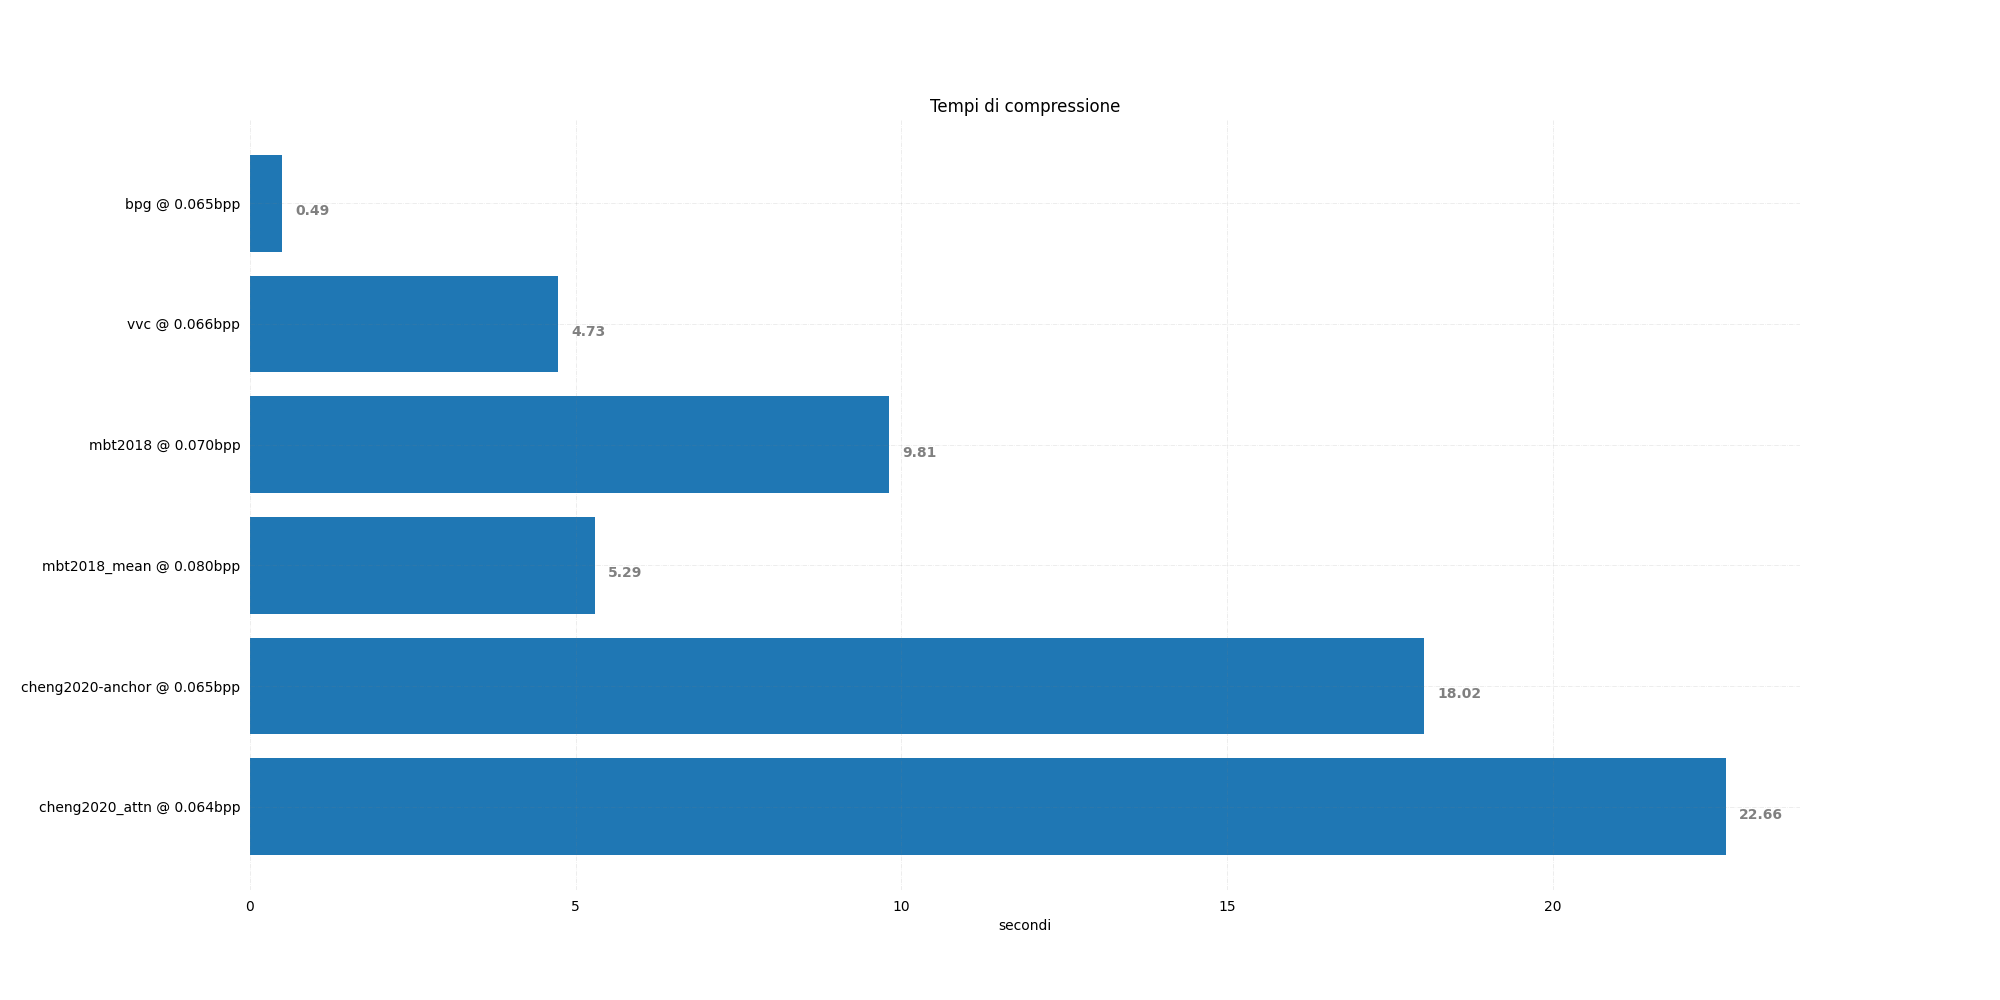
\includegraphics[width=1\textwidth]{Immagini/METRICS/times@0.07bpp.png}
    \caption{Tempi di compressione a 0.07 bpp}
    \label{fig:times07}
\end{figure}
\newpage
\begin{figure}[!h]
    \centering
    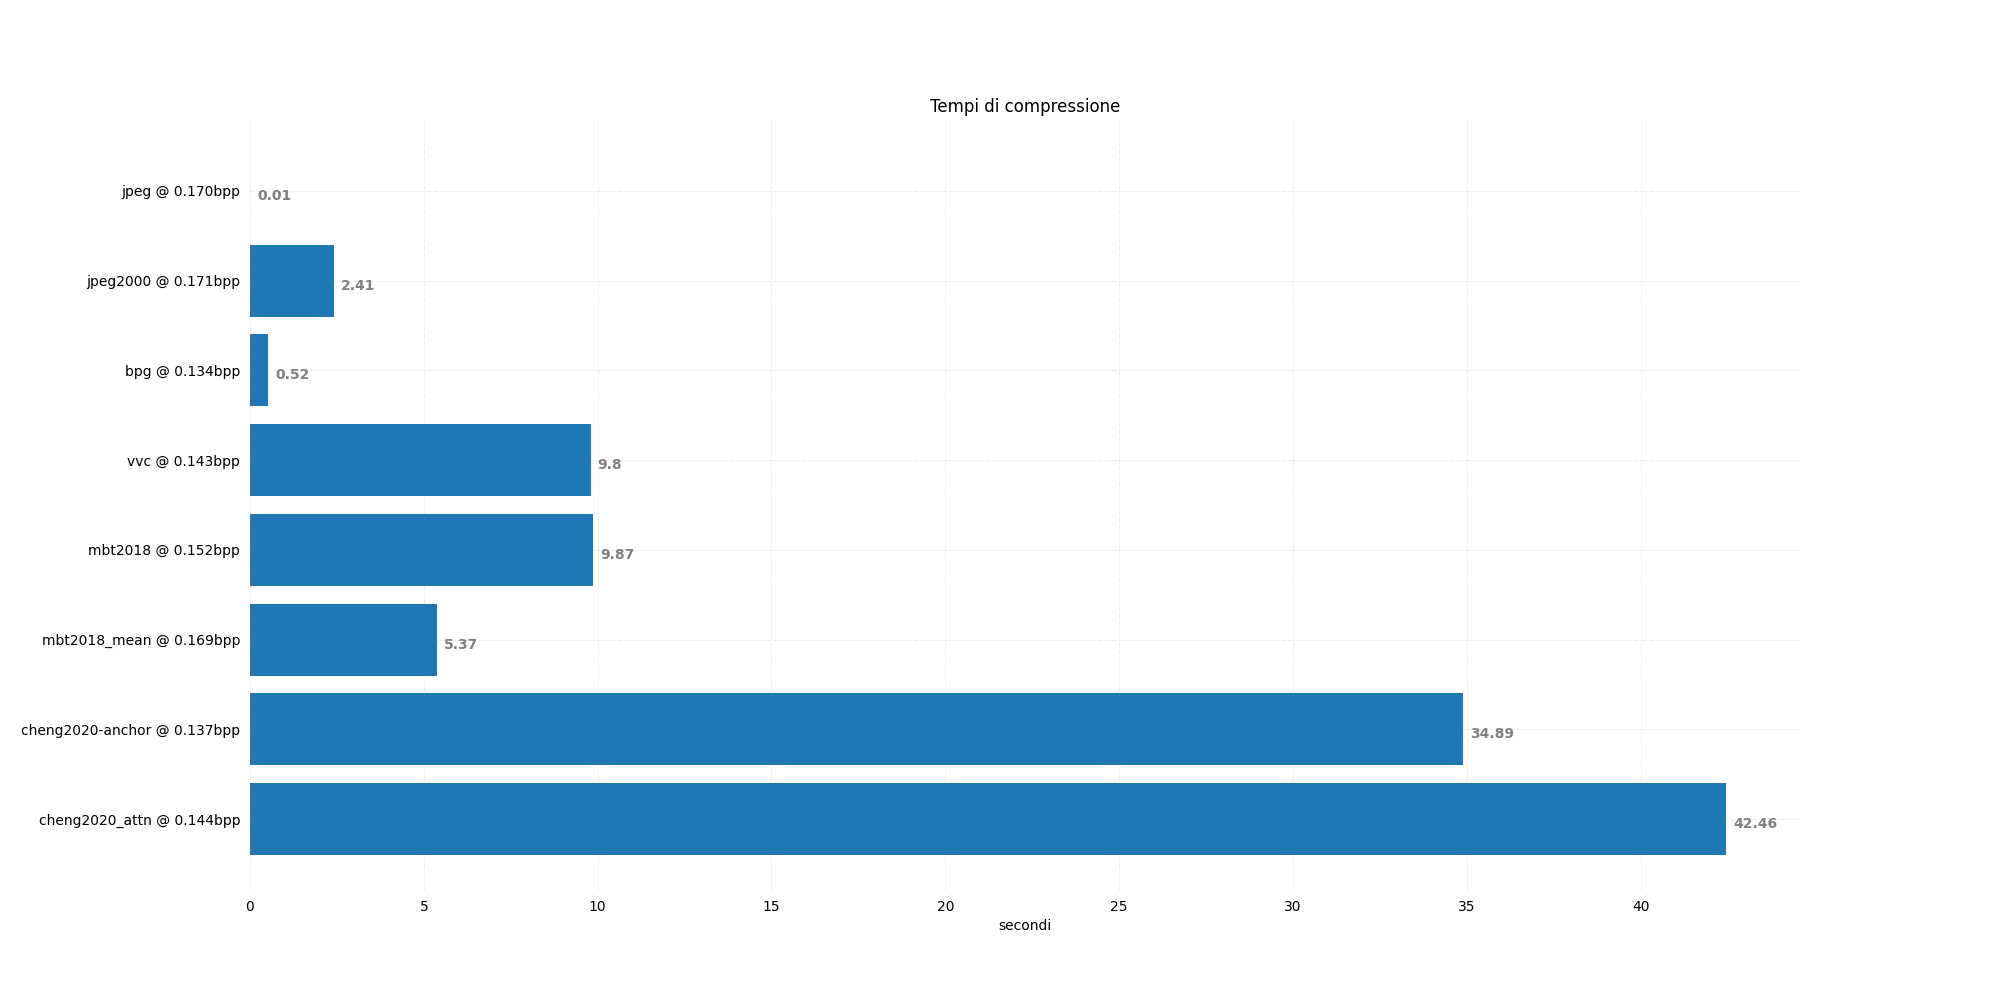
\includegraphics[width=1\textwidth]{Immagini/METRICS/times@0.16bpp.png}
    \caption{Tempi di compressione a 0.16 bpp}
    \label{fig:times16}
\end{figure}
\hspace{0.5cm}
\begin{figure}[!h]
    \centering
    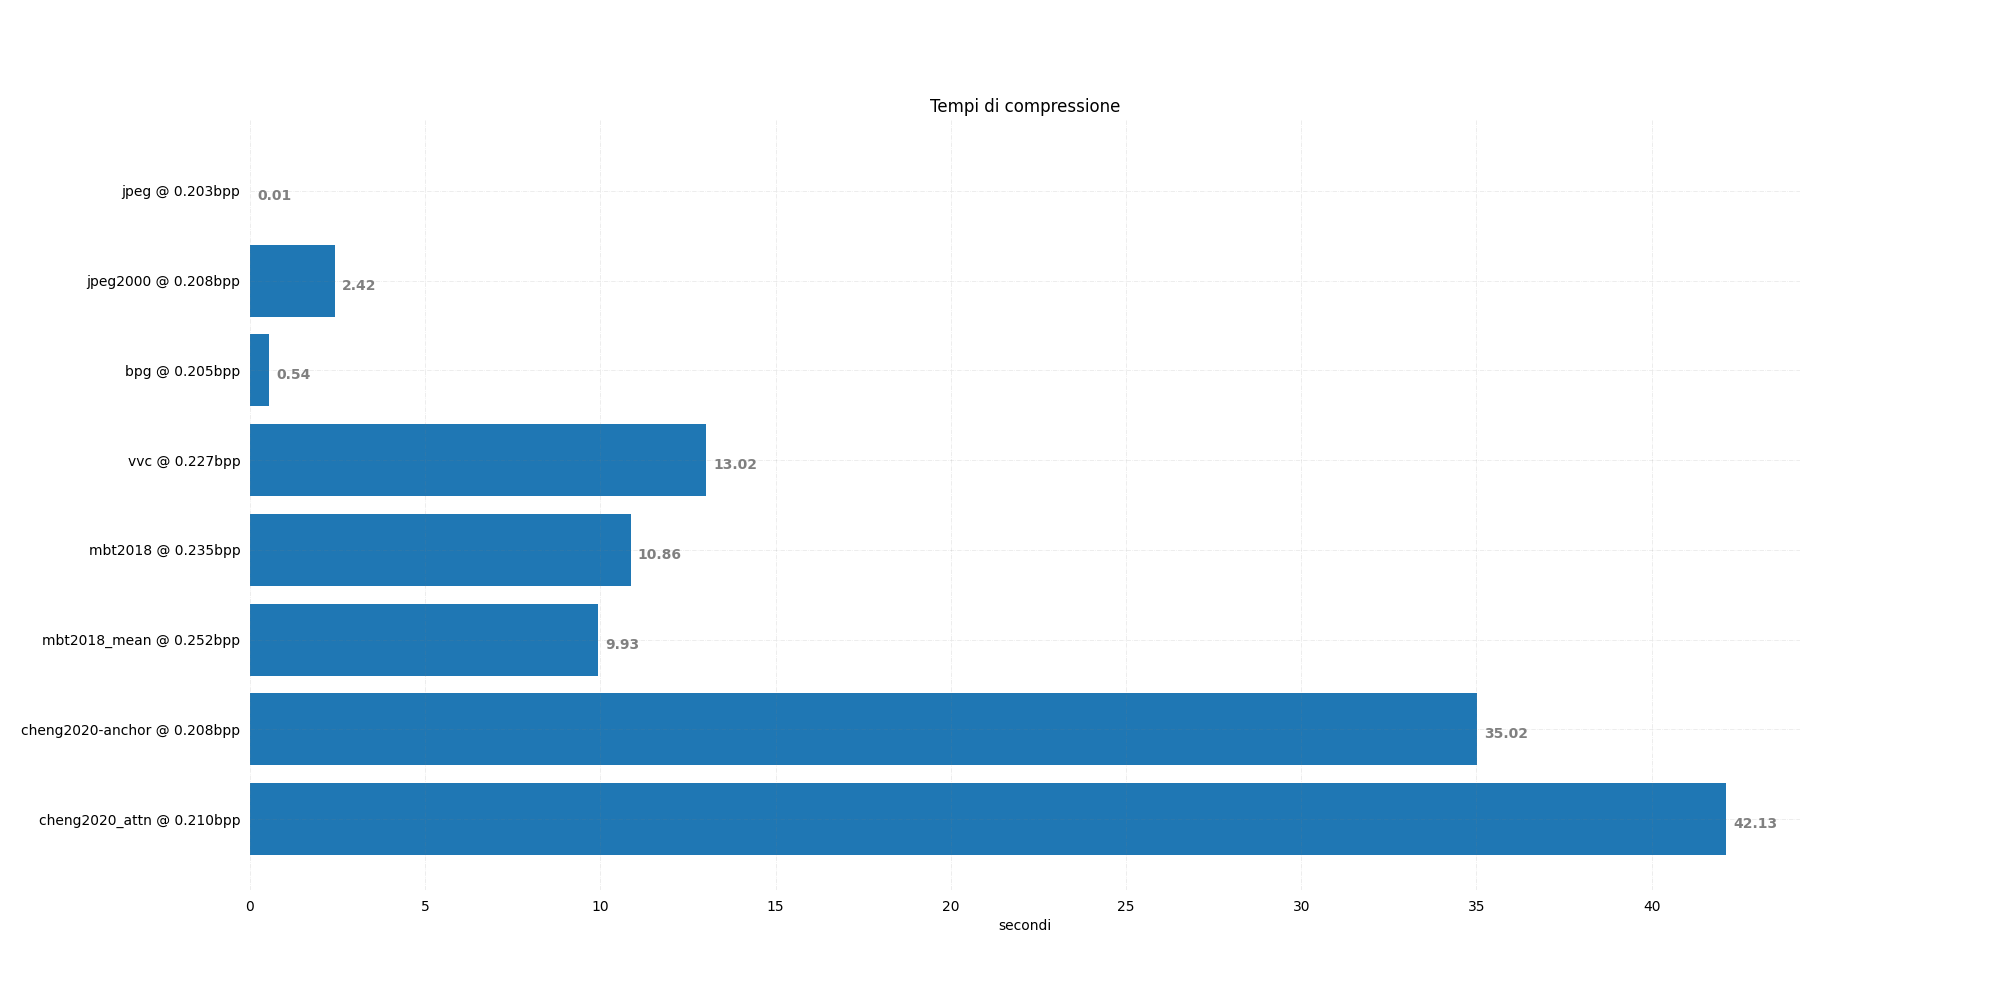
\includegraphics[width=1\textwidth]{Immagini/METRICS/times@0.21bpp.png}
    \caption{Tempi di compressione a 0.21 bpp}
    \label{fig:times21}
\end{figure}
\newpage
\begin{figure}[!h]
    \centering
    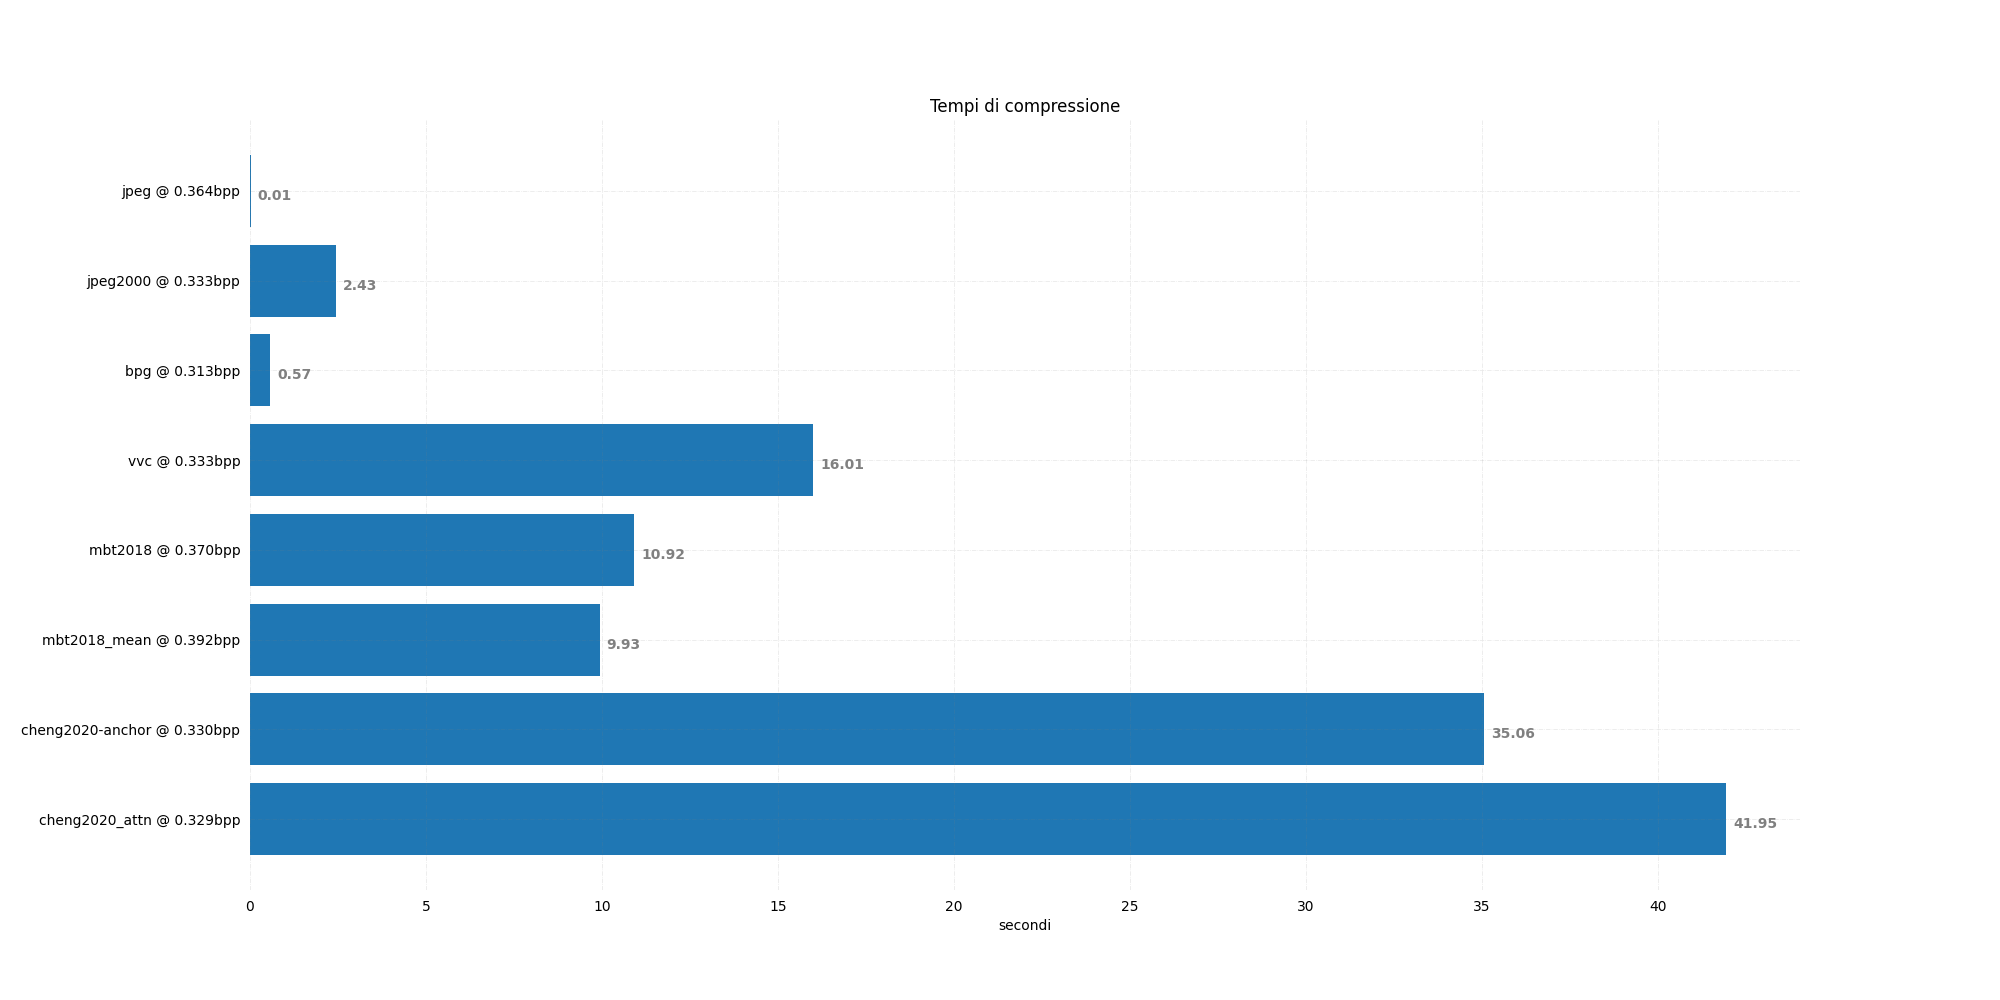
\includegraphics[width=1\textwidth]{Immagini/METRICS/times@0.34bpp.png}
    \caption{Tempi di compressione a 0.34 bpp}
    \label{fig:times34}
\end{figure}
\hspace{0.5cm}
\begin{figure}[!h]
    \centering
    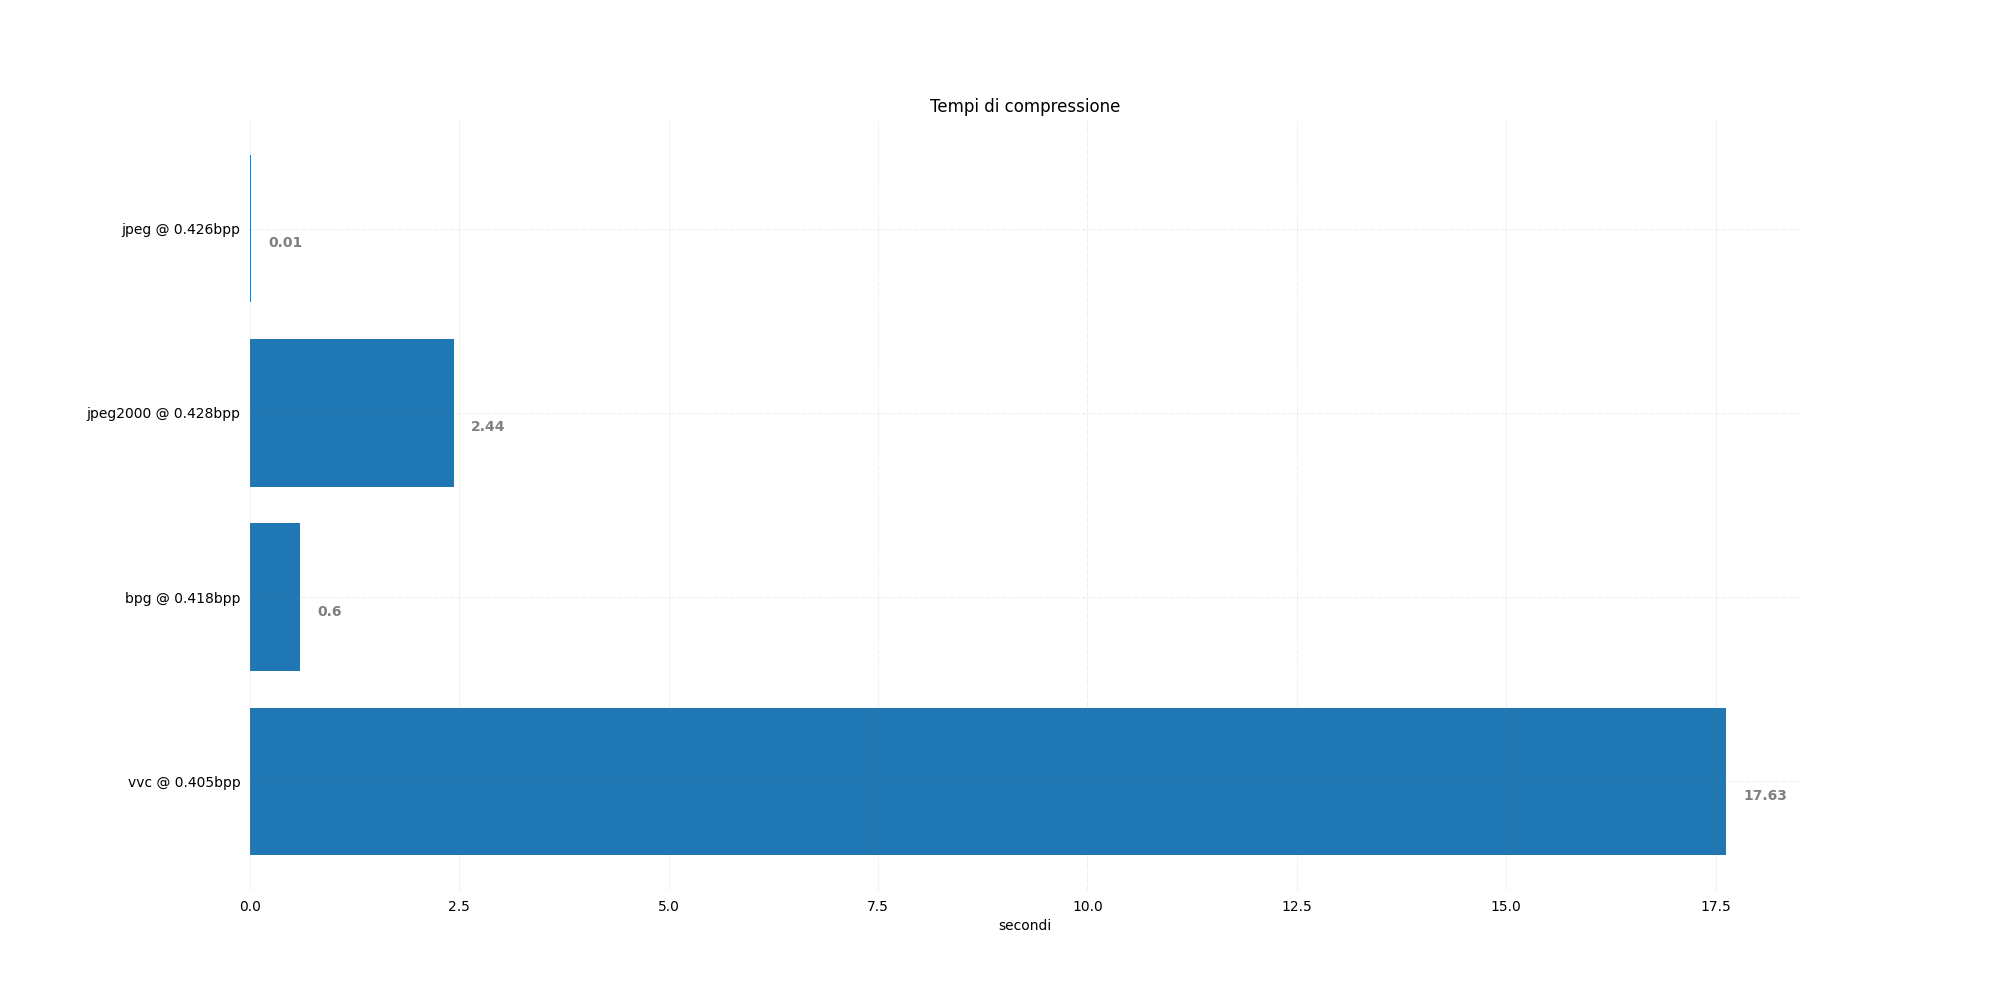
\includegraphics[width=1\textwidth]{Immagini/METRICS/times@0.41bpp.png}
    \caption{Tempi di compressione a 0.41 bpp}
    \label{fig:times41}
\end{figure}
\clearpage 
Come possiamo osservare nei grafici i tempi di compressione delle reti aumentano all’aumentare della qualità, i tempi di compressione dei metodi tradizionali invece non variano sensibilmente all’aumentare della qualità. Il codec VVC costituisce però un’eccezione a questo comportamento costante dei metodi tradizionali, in quanto possiamo vedere che il tempo aumenta all’aumentare della qualità. Questo comportamento si ha per la complessità di H.266, in quanto deve trovare il miglior metodo di compressione tra quelli a sua disposizione.\\
Passiamo ora a presentare le metriche di qualità dell’immagine, partiamo dal grafico del PSNR \ref{fig:PSNRGraph}, come possiamo vedere nel grafico, la migliore qualità di compressione si ha con il codec VVC, seguito poi da Cheng 2020, Ballé 2018, BPG, JPEG 2000 ed infine JPEG. H.266 si conferma quindi l’attuale stato dell’arte per la compressione di immagini osservando il grafico del PSNR, che ricordiamo essere una metrica oggettiva.\\
\begin{figure}[!h]
    \centering
    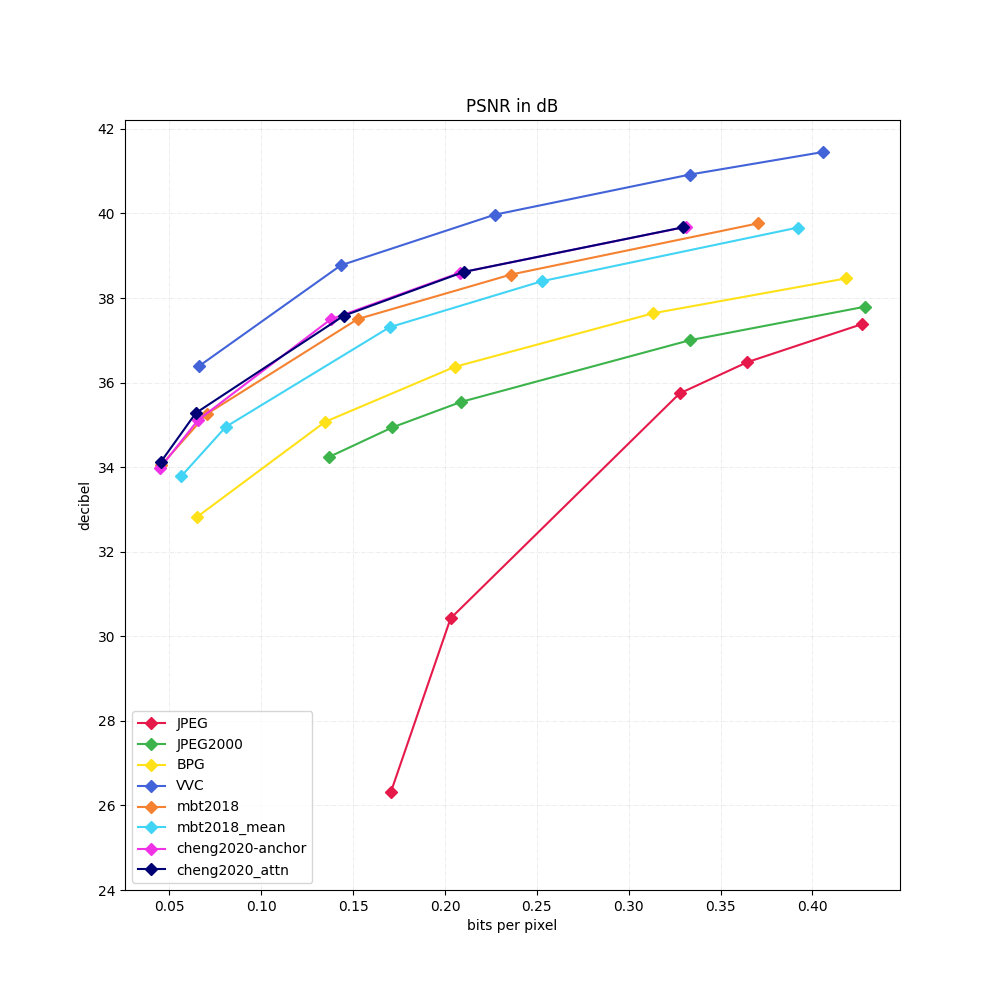
\includegraphics[width=0.9\textwidth]{Immagini/METRICS/PSNR.png}
    \caption{Grafico PSNR}
    \label{fig:PSNRGraph}
\end{figure}\\
Il prossimo grafico che andremo a commentare è il grafico dell’MS-SSIM \ref{fig:MSSSIMGraph}, in questo grafico possiamo osservare come JPEG, JPEG 2000 e BPG si confermino i metodi che forniscono le qualità di compressione peggiori. Diversamente da quanto osservato nel grafico del PSNR, secondo questo grafico il miglior metodo di compressione è Cheng2020, seguito da Balle2018 e come terzo abbiamo VVC.\\
Ricordiamo che l’MS-SSIM è invece una metrica che cerca di replicare la valutazione del sistema visivo umano.\\
\begin{figure}[!h]
    \centering
    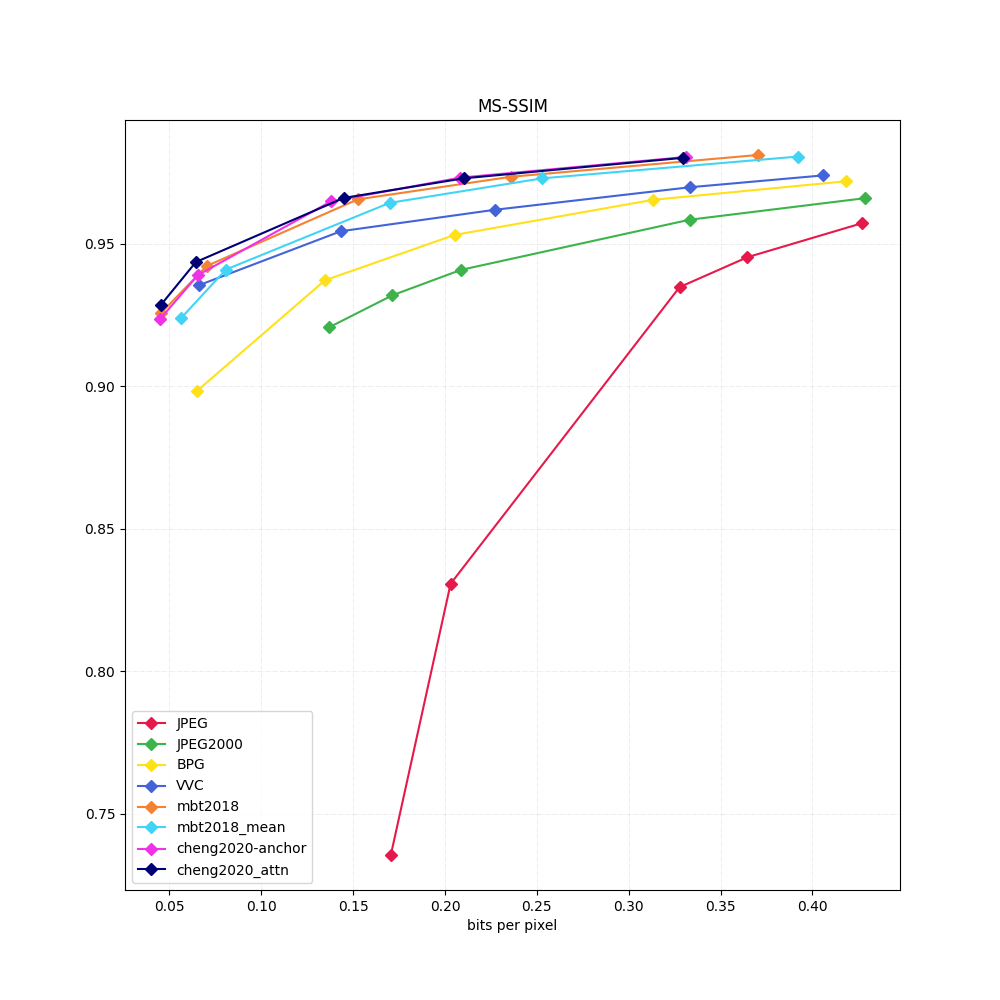
\includegraphics[width=0.9\textwidth]{Immagini/METRICS/MS-SSIM.png}
    \caption{Grafico MS-SSIM}
    \label{fig:MSSSIMGraph}
\end{figure}\\
L’ultima metrica è invece la più recente, andiamo ora a presentare i risultati presenti nel grafico della metrica LPIPS con AlexNet \ref{fig:LPIPSGraph}. Come possiamo vedere in questo grafico VVC si conferma il metodo migliore, seguito da Cheng2020, Ballé2018, BPG, JPEG 2000. Per quanto riguarda JPEG otteniamo un comportamento inaspettato in quanto i primi due punti sono in linea con le aspettative, il successivo invece è vicino a JPEG200 e gli ultimi due lo superano addirittura.\\
Questo comportamento ci ha sorpreso in quanto ci aspettavamo che la qualità percepita fosse vicina a quella di JPEG 2000 ma non che la superasse.\\
\begin{figure}[!h]
    \centering
    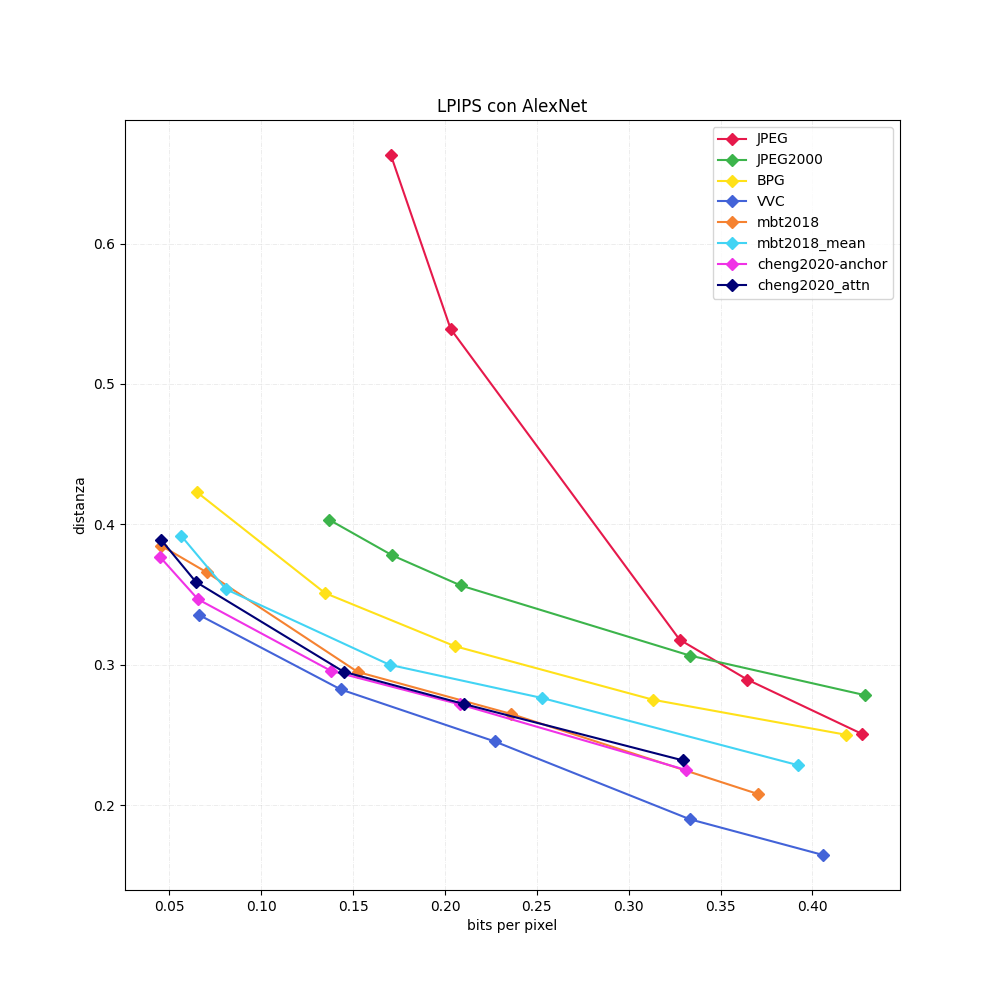
\includegraphics[width=0.9\textwidth]{Immagini/METRICS/LPIPS.png}
    \caption{Grafico LPIPS con AlexNet}
    \label{fig:LPIPSGraph}
\end{figure}\\
Dopo aver presentato e commentato questi grafici ci sentiamo di affermare che le reti da noi valutate svolgono un lavoro molto buono, che supera i metodi di compressione tradizionali più usati. Non riescono però ancora a superare il codec VVC che attualmente rimane lo stato dell’arte per la compressione di immagini.\\
